%%%%%%%%% NEW SECTION: GRAPHICAL USER INTERFACE %%%%%%%%%

\section{Graphical User Interface}
The graphical user interface, or GUI, is the part of the program where the user interacts with the software. \verb!wxPython! and \verb!wxFormbuilder! were used to make the GUI. In it the user can define the requirements for the measurement and the program will then compute the scan length and stepsize which are needed to meet the requirements.

\subsection{Walkthrough}

To start the program, click the icon or in the command window go to the correct folder and type \verb!python program_stepintegrate.py!. A window pops up with four frames, a `Welcome' frame, one to set the correct switches on the SR510 lock in amplifier, one for the measurement input and a frame to start the actual measurement.

\subsubsection{Welcome}

\begin{figure}[!ht]
 \begin{center}
  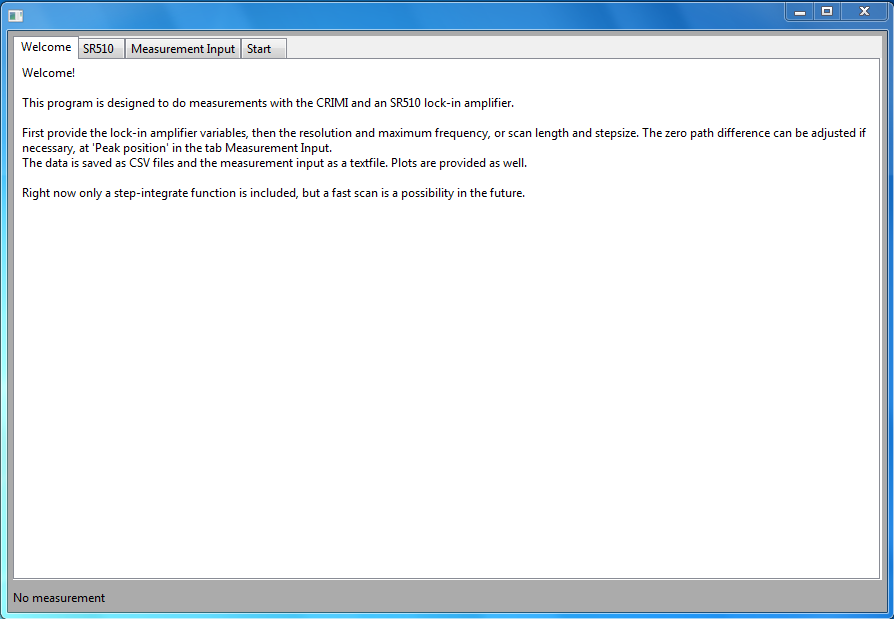
\includegraphics[width=0.8\textwidth]{figures/gui1}
  \caption{The GUI, frame 1: Welcome.}
  \label{fig:gui1}
 \end{center}
\end{figure}

Figure \ref{fig:gui1} shows the welcome screen with a short explanation on how to use this program. For the longer explanation, please read on.

\subsubsection{Setting the SR510 Lock In Amplifier}\label{subsub:lockin}

\begin{figure}[!ht]
 \begin{center}
  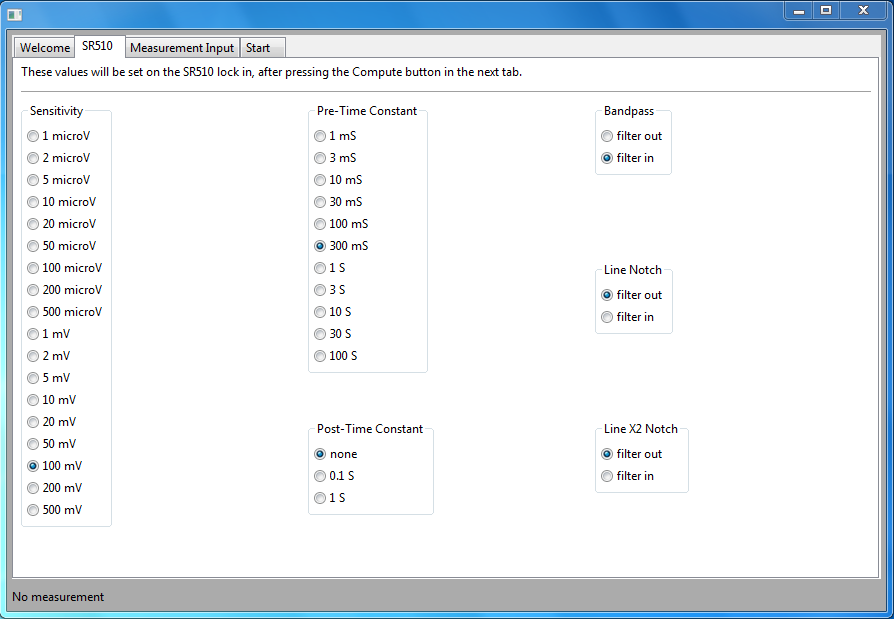
\includegraphics[width=0.8\textwidth]{figures/gui2}
  \caption{The GUI, frame 2: Setting the SR510 lock in amplifier.}
  \label{fig:gui2}
 \end{center}
\end{figure}

The second frame of the program, as shown in figure \ref{fig:gui2}, gives the most important features of the SR510 to set for the measurement. These settings are saved in a text file when the measurement is saved (see section \ref{subsub:saving} for more on saving the measurement data). Other settings can be changed on the lock in amplifier directly, but these settings will not be saved in the text file. The commands will be sent to the device after the button `Compute values and set SR510' in frame 3 has been pressed. The settings shown are the default values.

\subsubsection{Setting the Parameters for the Measurement}

\begin{figure}[!ht]
 \begin{center}
  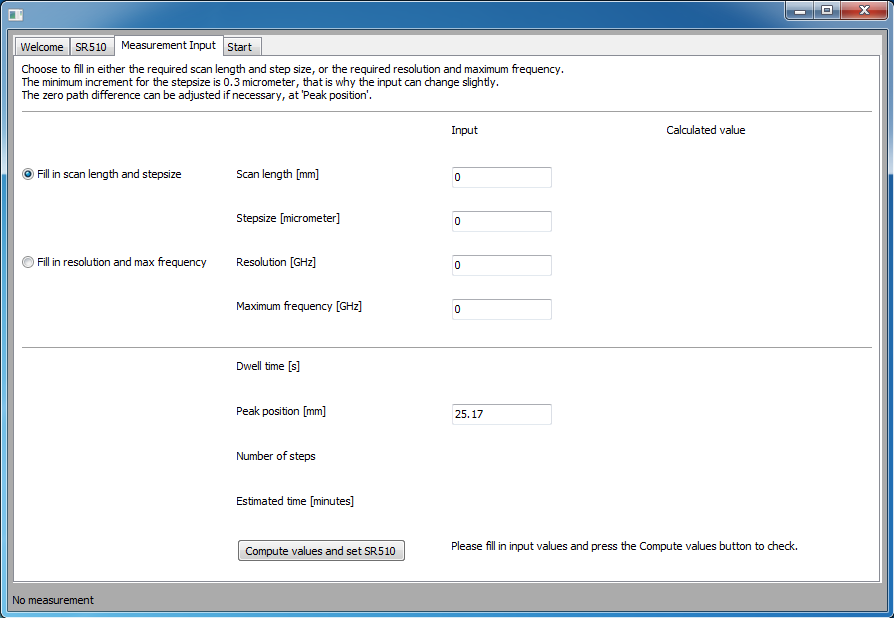
\includegraphics[width=0.8\textwidth]{figures/gui3}
  \caption{The GUI, frame 3: Setting the desired measurement input.}
  \label{fig:gui3}
 \end{center}
\end{figure}

In this frame (see figure \ref{fig:gui3}) the measurement input can be set. One can choose to fill in either the scan length and stepsize or the resolution and maximum frequency. The program converts this after pressing the `Compute values' button.

The discrepancies in the entered values and the computed values are because of the minimum stepsize of 0.3 micrometer that the stage can make. The code is designed such that the rounded values always represent a higher accuracy in the measurements than the provided values (e.g. smaller stepsize or higher resolution).

The zero bias point is experimentally found to be at a distance of 25.17 cm from the beginning of the stage. It can be adjusted easily by changing the value for the `Peak position'. Figure~\ref{fig:peakposition} shows a scan around the center, taken at a later moment. This plot shows that the value of 25.17 is not far off. A higher precision can be attained by tuning this zero bias point.

\begin{figure}[!ht]
 \begin{center}
  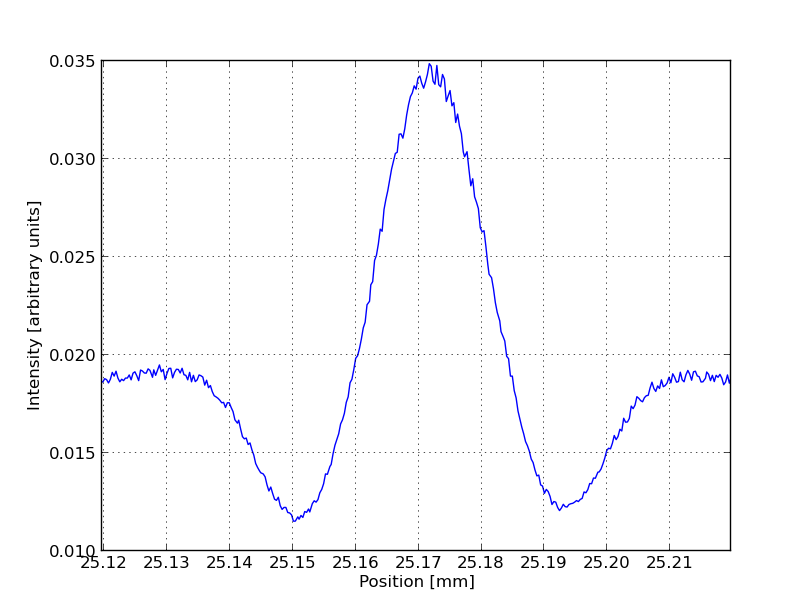
\includegraphics[width=\textwidth]{figures/peakposition}
  \caption{Experimental determination of the zero bias position.}
  \label{fig:peakposition}
 \end{center}
\end{figure}


\subsubsection{Starting and Saving the Measurement}\label{subsub:saving}

In the last frame, figure~\ref{fig:gui4}, the measurement can be started by pressing the `Start' button. In this frame two plots are updated continually: the interferogram as measured in the upper window, and the Fourier transform with a Hann apodization function in the lower window. These can be used to track the progress of the measurement. If necessary, the measurement can be stopped by pressing the `Abort' button.

In the grey band under every frame the status is given. The possibilities are `No measurement', `Measurement started', 'Measurement aborted', or `Measurement finished'. After a succesful measurement, the status will stay at `Measurement finished', and a new measurement can be started.

Saving is done by pressing the `Save' button. All files are saved with the exact time and date from when the measurement was started in the name; this prevents the possibility of overwriting earlier measurements. Three plots are saved as \verb!png!: the original interferogram, the Fourier transformed data without a windowing function and the Fourier transformed data with a Hann apodization function. These data points are also saved in two \verb!csv! files, one with the original data, and one with the transformed data. Lastly a textfile with the parameters used in the measurement is saved.

\begin{figure}[!ht]
 \begin{center}
  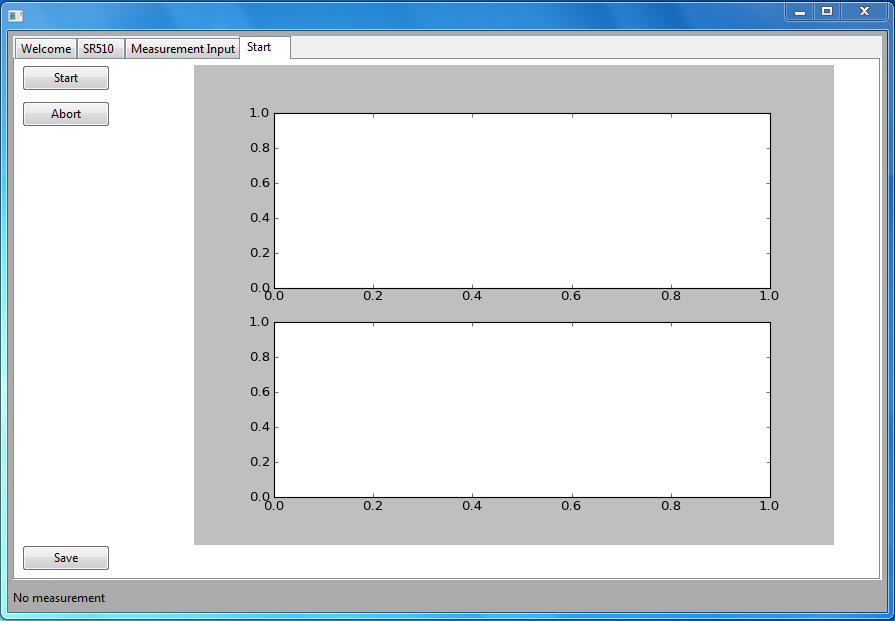
\includegraphics[width=0.8\textwidth]{figures/gui4}
  \caption{The GUI, frame 4: Starting the measurement, a plot of the measured points, and saving the data afterwards.}
  \label{fig:gui4}
 \end{center}
\end{figure}
